\chapter*{Summary}
\addcontentsline{toc}{chapter}{Summary}
\setheader{Summary}


\section*{Introduction and Motivation}
Nuclear materials are highly complex multiscale, multiphysics systems and there has been a increasing interest in adopting multiscale approach to better simulate the behaviour of nuclear materials. Material behaviour is influenced by many different physics, for example, mechanics such as dislocations, cracking, stress driven diffusion; chemistry such as corrosion, oxidation, reactive transport; heat conduction such as species transport, melting, precipitation; etc. Furthermore, the phenomena at the atomistic and micro scales drive the macro scale response. The multiscale modelling approach aims at using information from smaller scales to inform the models at increasing length scales and helps in effective prediction of performance of nuclear materials \cite{STAN200920}.

The evolution of the composition of nuclear materials due to irradiation plays a significant role in driving the above mentioned phenomena and thermochemical equilibrium calculations help in providing the information such as material properties and boundary conditions for continuum and mesoscale codes. As a result, recent trends in modelling and simulation of nuclear materials have exhibited a desire to couple thermochemical equilibrium codes within multiphysics frameworks.

Many emerging nuclear technologies such as the Molten Salt Reactor (MSR) use high temperature fluids such as molten fluoride/chloride salts, which lead to corrosion of the metal containment leading to problematic behaviours during the reactor operations. Corrosion is an electrochemical process composed of oxidation and reduction reactions which are defined by the thermodynamics and kinetics of the reactions. While thermodynamics tells us whether or not a material may corrode, kinetics tells us how quickly the material will corrode. This corrosion behaviour is also significantly affected by the material microstructure and predicting corrosion therefore requires a multiphysics approach that can couple quantitative electrochemistry models of corrosion and chemical reactions with thermochemical equilibrium computations. The \texttt{Multiphysics Object Oriented Simulation Environment (MOOSE)} developed by the Idaho National Laboratory provides a framework for multiphysics simulations but lacks the tools for predicting corrosion at the microstructure scale. A new \texttt{MOOSE}-based tool, \texttt{Yellowjacket}, is currently being developed to perform such simulations and provide quantities such as the rate of material loss, corrosion product production, and precipitate production in liquid. As part of \texttt{Yellowjacket}, a thermochemical equilibrium solver is being developed to quantitatively provide quantities of interest, for example chemical potential of stable species, by using the principles of computational thermodynamics.

\section*{MOOSE Framework}
    The \texttt{Multiphysics Object-Oriented Simulation Environment (MOOSE)} is a tool for solving complex coupled Multiphysics equations using the finite element method. \texttt{MOOSE} uses an object-oriented design to abstract data structure management, parallelism, threading and compiling while providing an easy to use interface targeted at engineers that may not have a lot of software development experience. \texttt{MOOSE} provides extreme scalability and flexibility when compared to other finite element method (FEM) frameworks. For instance, \texttt{MOOSE} has the ability to run extremely complex material models, or even third-party applications within a parallel simulation without sacrificing parallelism. This capability is in contrast to what is often seen in commercial packages, where custom material models can limit the parallel scalability, forcing serial runs in the most severe cases \cite{gaston2015physics,moose-web-page}.

    The design goal of \texttt{MOOSE} is to give developers ultimate control over their physical models and applications. Designing new models or solving completely new classes of problems is accomplished by writing standard C++ source code within the framework?s class hierarchy. Scientists and engineers are free to implement completely new algorithms using pieces of the framework where possible, and extending the framework?s capabilities where it makes sense to do so. Commercial applications do not have this capability, and instead opt for either a more rigid parameter system or a limited application-specific metalanguage \cite{moose-web-page}.
    
    \subsection*{Yellowjacket}
    The \texttt{MOOSE} framework currently lacks a quantitative tool for corrosion prediction at the microstructure scale. To bridge this gap, a new mesoscale framework for thermodynamics based modelling of corrosion in advanced reactor materials namely \texttt{Yellowjacket} is under development. \texttt{Yellowjacket} is a \texttt{MOOSE} based application that couples quantitative models of corrosion with thermodynamic and kinetic databases to predict the rate of material loss, corrosion product production and precipitate production for advanced reactors. Yellowjacket relies on phase field models for structure evolution, coupling it with Poisson equation for electrostatics, fracture models and thermochemical equilibrium solvers to provide a holistic  environment for corrosion modelling and simulation.
    
    \subsection*{Thermochemistry in Yellowjacket}
    The composition of nuclear materials constantly evolves due to irradiation. This results in an evolution of the material properties which constantly change as the stable phases in the system evolve as a function of temperature, pressure and composition of the system. Thermodynamic computations provide quantitative capabilities for predicting phase distribution and chemical potentials in fuels and other materials and coupling thermodynamics with other multiphysics codes can provide material properties (e.g. heat capacity, oxygen to metal ratio) and boundary conditions as the composition evolves thereby improving the predictions of nuclear material performance and improving safety.
    
    \begin{figure}
        \centering
        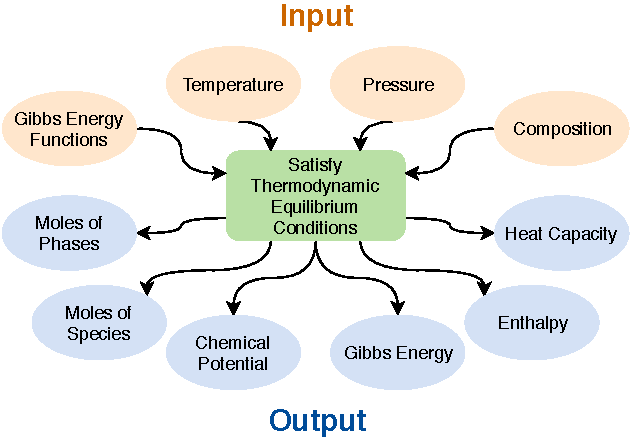
\includegraphics[width=0.75\textwidth]{figures/Thermodynamics.pdf}
        \caption{Input and output parameters of thermodynamic equilibrium calculations.}
        \label{fig:Thermod}
    \end{figure}
    
    As shown in fig.~\ref{fig:Thermod}, by relying on the fundamental laws of thermodynamics, equilibrium computations use the system information, namely, Gibbs energy functions of the species that can be present in the system, temperature, pressure and composition to provide quantities such as the stable phases and species, Gibbs energy of the system, chemical potentials of the species and can be used to provide information such the enthalpy, heat capacity, etc. A detailed description of the thermodynamic equilibrium computation is provided in the following section.
    
    The thermochemical equilibrium solver in \texttt{Yellowjacket} leverages the experience from the development of a similar code \texttt{Thermochimica} \cite{PIRO2013266}. By using the standard tools and libraries being used in \texttt{MOOSE}, the aim is to develop an improved thermochemical equilibrium solver for complete integration with other \texttt{MOOSE} based codes.
    
\section*{Thermochemical Equilibrium}
    Thermochemical equilibrium calculations are based on minimising the integral Gibbs energy of a closed system at constant temperature and hydrostatic pressure. From a numerical point of view, the objective of computing thermochemical equilibrium is to determine a unique combination of phases and their composition that yields a global minimum in the integral Gibbs energy subject to various linear and non-linear equality constraints.
\subsection*{Gibbs energy}
    The integral Gibbs energy of a multicomponent multiphase system is represented as
    \begin{equation*}
        G = RT \left ( \sum_{\lambda=1}^{\Lambda} n_{\lambda} \sum_{i=1}^{N_{\lambda}}x_{i({\lambda})}\tilde{\mu}_i + \sum_{\omega=1}^{\Omega} n_{\omega} \tilde{\mu}_{\omega} \right )
    \end{equation*}
    where, $R$ [\si{\joule \per \mole \per \kelvin}] is the ideal gas constant, $T$ [\si{\kelvin}] is the absolute temperature, $N_{\lambda}$ denotes the number of species in the solution phase $\lambda$ and $x_{i({\lambda})}$ represents the mole fraction of species $i$ in solution phase $\lambda$. $\Lambda$ and $\Omega$ represent the number of stable solution phases and stoichiometric phases respectively and the number of moles of the solution phase $\lambda$ and stoichiometric phase $\omega$ are denoted by $n_\lambda$ and $n_\omega$ [\si{\mole}] respectively. Finally, $\tilde{\mu}_i$ and $\tilde{\mu}_j$ represent the dimensionless chemical potential of species $i$ in solution phase $\lambda$ and stoichiometric phase $\omega$ respectively. 
    
    The chemical potential is a measure of the change of the Gibbs energy of a system by the introduction of a substance. Mathematically, the chemical potential of a species $i$ is defined as 
    \begin{equation*}
        \mu_i = {\left (\frac{\partial G}{\partial n_i} \right )}_{T,P,n_{j \neq i}}
    \end{equation*}
    and for the species of an ideal phase, the chemical potential incorporates the reference Gibbs energy of pure species,$g_{i(\lambda)}^0$, and the entropic contribution due to mixing as a function of its mole fraction.
    \begin{equation*}
        \mu_i = g_{i(\lambda)}^0 + \ln x_{i(\lambda)}
    \end{equation*}
    For non-ideal solution phases, the chemical potential also includes the partial molar excess  Gibbs energy of mixing, $g_{i(\lambda)}^{ex}$, to account for non-ideal mixing
    \begin{equation*}
        \mu_i = g_{i(\lambda)}^0 + \ln x_{i(\lambda)} + g_{i(\lambda)}^{ex}
    \end{equation*}
    
    While the chemical potential of stoichiometric phases does not include a composition dependent term, the partial molar excess Gibbs energies of mixing for non-ideal solution models depend on the mixing model employed. Some of these models include the Modified Quasichemical Model, the Compound Energy Formalism, etc.

\subsection*{Conditions for thermochemical equilibrium}
    	Achieving thermochemical equilibrium in a system requires satisfaction of several conditions which are as follows:
	\subsubsection{Necessary conditions}
    	\begin{enumerate}\compresslist
        		\item \emph{Conservation of mass} requires that the mass of element $j$, $b_j$, must satisfy the following mass balance equation 
            	\begin{equation*}
                		b_j = \sum_{\lambda=1}^{\Lambda} n_{\lambda}\sum_{i=1}^{N_{\lambda}}x_{i({\lambda})}{\nu}_{i,j} +  \sum_{\omega=1}^{\Omega} n_{\omega}{\nu}_{\omega}
            	\end{equation*}
            	where, ${\nu}_{i,j}$ and ${\nu}_{\omega}$ represent the stoichiometric coefficients of element $j$ in solution phase species $j$ and stoichiometric phase $\omega$ respectively.
        		\item \emph{Gibbs' phase rule} which defines the thermodynamic degrees of freedom of the system must also be     satisfied
            	\begin{equation*}
                		F=C-\Phi + 2 + \Xi
            	\end{equation*}
            	where, $F$ represents the degrees of freedom, $C$ denotes the number of components in the system, $\Phi$ denotes the number of phases and $\Xi$ denotes the electrochemical terms.
        		\item \emph{Gibbs' criteria} for equilibrium requires that the Gibbs energy of a system be at a global equilibrium. In equivalent terms, the chemical potential for each system component must have the same value in all stable phases within the system \cite{HILLERT198131}, where the chemical potential of any constituent in a stable phase can be defined as a linear function of the element potentials, $\Gamma_j$, as
            	\begin{equation*}
		        \mu_{i} = \sum_{j=1}^C \nu_{i,j} \Gamma_j                 
            	\end{equation*}
    	\end{enumerate}

	\subsubsection*{Sufficient conditions}
    	The necessary conditions for thermodynamic equilibrium require that the chemical potentials of all stable solution phase species and stoichiometric phases abide by the above equality, which is equivalent to Gibbs energy of the system being at a local minimum, and that the conservation of mass and the Gibbs phase rule are satisfied. The sufficient condition requires that all the metastable phases abide by the following conditions 
    	\begin{equation*}
        		\pi_{\lambda} = \min_{\lambda} \sum_{i=1}^{N_{\lambda}}x_{i({\lambda})} \left (\mu_{i({\lambda})} - \sum_{j=1}^C \nu_{i,j}\Gamma_j \right )
    	\end{equation*}
    	i.e., there must exist a Gibbs' plane such that the element potentials lie on the plane and the chemical potentials of all the species lie on or above the plane and the mole fraction of the species must satisfy the following constraints
	\begin{equation*}
        		\begin{aligned}
            		\sum_{i=1}^{N_{\lambda}}x_{i({\lambda})} = 1 \\
			x_{i({\lambda})} \geq 0 \;\; \forall i
        		\end{aligned}
    	\end{equation*}
    	i.e., the sum of mole fraction of all the species in a phase $\lambda$ must be unity and that the individual mole fractions must be greater than or equal to zero.
    
    	The aforementioned conditions are used in the Gibbs energy minimiser to find a unique combination of phases that are stable in the system. The computational structure of the code has been presented in the following section.
	
\section*{Gibbs Energy Minimiser}
\subsection*{Computational Structure}
  	A top level overview  of the  Gibbs energy minimisation code has been shown in fig.~\ref{fig:gemsolverintro}. The inputs required for the computation are provided at the parsing and input stages which is followed by a linear solver to provide initial assemblage. Subsequently, a non-linear minimisation routine finds the final assemblage which is verified using the global optimisation module thus obtaining the final output.
    	\begin{figure}[h]
        		\centering
        		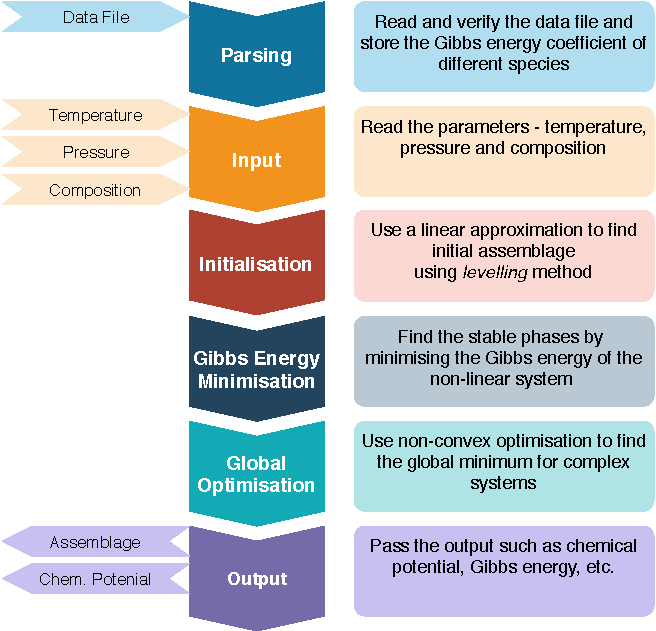
\includegraphics[width=0.75\textwidth]{figures/YJ_structure.pdf}
        		\caption{Computational structure of a Gibbs energy minimisation program}
        		\label{fig:gemsolverintro}
    	\end{figure}
    
\subsection*{Software Overview}
    	For the sake of completeness, a short description of the individual modules is presented in this section. However, this is not an exhaustive description of the  code and must not be treated as such.
    	\subsubsection*{Data File Parsing}
    	Calculation of thermodynamic equilibrium requires a thermodynamic database, which provides Gibbs energy terms of different species in addition to models representing non-ideal behaviour. These thermodynamic databases are developed using the well established CALPHAD method \cite{liu_wang_2016} and are available in different formats, the most commonly used being ThermoCalc (*.tdb) and ChemSage (*.dat) data file formats, which are generated by the commercial software ThermoCalc \cite{ANDERSSON2002273} and FactSage \cite{BALE201635}, respectively. Data file parsing allows the extraction of free energy expressions from *.dat thermodynamic database files (ChemSage format).
	
	\subsubsection*{System Inputs}
    Computation of thermodynamic equilibrium also requires system information such as temperature, pressure and elemental composition of the system. For computations on a finite element mesh, this information is required for every element at each time step. The system inputs to \texttt{Yellowjacket} can be provided either through a \texttt{MOOSE} input file for standalone computations or by passing the required information in the function call when \texttt{Yellowjacket} is coupled with other codes such as \texttt{Bison} and \texttt{Marmot}.
    
    	\subsubsection*{Initialisation}
    	Thermodynamic solvers require an initial estimate of molar quantities of species and phases. To this aim, a general estimating procedure called \emph{levelling} was developed by Eriksson and Thompson \cite{ERIKSSON1989389}. At every iteration, the levelling algorithm accelerates convergence by providing an estimated phase assemblage that focuses on only the dominant species. These are typically not equivalent to the final equilibrium state, but a good initial approximation. 

    	Mathematically, levelling converts the non-linear optimisation problem into a linear optimisation problem with the objective of systematically adjusting fixed combinations of phases, subject to linear equality and inequality constraints, to progressively make the Gibbs energy of the system more negative. An advantage of levelling is that the number of iterations required to achieve convergence does not increase rapidly with the number of system components. Moreover, the initialisation of the non-linear solver using the phase assemblage calculated by the levelling solver can greatly improve the rate of convergence.
    
    	While levelling provides great initial assemblage, in many cases, such as the time dependent problems, other initialisation methods can be used to further reduce the computational time required by the non-linear solver. A couple of these techniques have been studied by Piro \cite{Piro17} and include the use of assemblage from the preceding time step or from the neighbouring elements based on the principle of continuum. Though not yet implemented in \texttt{Yellowjacket}, these methods will be of significant interest in future as it can provide significant speed gains compared to re-initialisation using levelling at each time step.
	
	\subsubsection*{Gibbs Energy Minimisation}
    	The linear solver, though an excellent initialisation algorithm, rarely provides the actual assemblage of the system under consideration. Obtaining the final assemblage requires minimisation of a non-linear objective function representing the integral Gibbs energy of the system subject to mass balance and Gibbs phase rule constraints. Gibbs energy minimisation introduced by White \textit{et al.} \cite{White:58} is the universally used algorithm to perform the non-linear optimisation for obtaining thermochemical equilibrium in complex systems. 
    
    	In mathematical terms, Gibbs energy minimisation is widely performed using using the method of Lagrange multipliers that simultaneously minimises the integral Gibbs energy and the residuals of mass balance equations. This results in a system of linearised equations that can be written in matrix form as \cite{Piro11b}
    	\begin{equation*} \label{eqn:GEMintro}
        		\mathbf{H} \cdot \boldsymbol{\pi} = \boldsymbol{\zeta}
    	\end{equation*}
    	where $\boldsymbol{\pi}$ and $\boldsymbol{\zeta}$ denote the  unknown and constraint vectors respectively, and the Hessian matrix ($\mathbf{H}$) can be written as \cite{Piro11b,White:58}
    	\begin{equation*}
        \mathbf{H} = 
        			\begin{bmatrix}
            		r_{j=1,k=1} & \dots & r_{j=1,k=C} & \phi_{j=1,\lambda=1} & \dots & \phi_{j=1,\lambda=\Lambda} & \nu_{j=1,\omega=1} & \dots & \nu_{j=1,\omega=\Omega} \\
            		\vdots & \ddots & \vdots & \vdots & \ddots & \vdots & \vdots & \ddots & \vdots \\
            		r_{j=C,k=1} & \dots & r_{j=C,k=C} & \phi_{j=C,\lambda=1} & \dots & \phi_{j=C,\lambda=\Lambda} & \nu_{j=C,\omega=1} & \dots & \nu_{j=C,\omega=\Omega} \\
            		\phi_{\lambda=1,j=1} & \dots & \phi_{\lambda=1,j=C} & 0 & \dots & 0 & 0 & \dots & 0 \\
            		\vdots & \ddots & \vdots & \vdots & \ddots & \vdots & \vdots & \ddots & \vdots \\
            		\phi_{\lambda=\Lambda,j=1} & \dots & \phi_{\lambda=\Lambda,j=C} & 0 & \dots & 0 & 0 & \dots & 0 \\
            		\nu_{\omega=1,j=1} & \dots & \nu_{\omega=1,j=C} & 0 & \dots & 0 & 0 & \dots & 0 \\
            		\vdots & \ddots & \vdots & \vdots & \ddots & \vdots & \vdots & \ddots & \vdots \\
            		\nu_{\omega=\Omega,j=1} & \dots & \nu_{\omega=\Omega,j=C} & 0 & \dots & 0 & 0 & \dots & 0 
        			\end{bmatrix}
    	\end{equation*}
    	where $C$ is the number of system components, $\lambda$ is an index of a solution phase, of which there are $\Lambda$ in the system, $\omega$ is an index of a stoichiometric phase, of which there are $\Omega$ in the system, $\nu_{i,j}$ is the stoichiometric coefficient of component $j$ in species $i$, and $r_{j,k}$ and $\phi_{j,\lambda}$ can be expressed as follows
    	\begin{equation*}
        		r_{j,k} = \sum_{\lambda = 1}^{\Lambda} \sum_{i = 1}^{N_\lambda} n_{i(\lambda)} \nu_{i,j} \nu_{i,k}
    	\end{equation*}
    	\begin{equation*}
        		\phi_{j,\lambda} = \sum_{i = 1}^{N_\lambda} n_{i(\lambda)} \nu_{i,j}
    	\end{equation*}
    	$N_\lambda$ is the number of species in phase $\lambda$, and $n_{i(\lambda)}$ is the number of moles of species $i$ in solution phase $\lambda$. Clearly, $r_{j,k}$ = $r_{k,j}$ and $\phi_{j,\lambda} = \phi_{\lambda,j}$, which yields a symmetric matrix for $\mathbf{H}$.
    
    	While finding a solution to eqn.~\ref{eqn:GEMintro} is relatively easy, the challenge arises due to the change in the size of Hessian $\mathbf{H}$ within a computation cycle. This change in size results from the addition/removal of phases in the system and requires the implementation of special strategies such as the ones discussed by Piro \cite{Piro17}. In addition, care must be taken in selecting the line search algorithms and proper use of Wolfe/Armijo conditions for choosing the step length can significantly improve the convergence of the non-linear solver.
    
	\subsubsection*{Global Optimisation}
    	The Gibbs energy functions of non-ideal phases are often non-convex, yielding multiple local minima after Gibbs energy minimisation. These local minima correspond to different compositions of phases that may be believed to be stable (e.g., a miscibility gap), which may not necessarily correspond to the true equilibrium composition. Finding the global minimum of this function among the many local minima within the domain space can be a daunting challenge, especially in large complex thermodynamic systems containing many highly non-ideal solution phases. Consequently, an inadequate numerical approach may lead one to the false belief of thermodynamic equilibrium, which may be far from the true equilibrium state \cite{Piro16}. While a large number of deterministic (e.g. branch and bound) and stochastic (e.g. particle swarm optimisation) methods are available in literature, none of them guarantees the ability of finding a global extremum of a non-convex function. Moreover, the computational effort associated with this task can increase very rapidly with the size of the system (i.e. the total number of species in the system). 
    
	\subsubsection*{Output}
    	The outputs produced at the end of the GEM and global optimisation include the moles of the different phases present in the system, the mole fraction of the species in each phase, Gibbs energy of the system, chemical potentials, etc. These outputs are either used by the electrochemistry module for corrosion or can be passed back to \texttt{MOOSE}.
	
\section*{Goals and Expected Outcomes}
The goal of this work is to develop a new state-of-the-art thermodynamic equilibrium code by leveraging the experience with the development and utilisation of \texttt{Thermochimica}. Though the thermodynamic equilibrium code is being developed within the corrosion modelling application \texttt{Yellowjacket}, it would be easily couple-able with other applications such as \texttt{Bison}. The code will rely on the \texttt{MOOSE} framework and exploit the multitude of mathematical and development tools of the framework to ensure that the code meets the stringent requirements of the nuclear industry. It must be mentioned that while \texttt{MOOSE} and other \texttt{MOOSE} based applications solve systems of partial differential equations (PDE) using finite element method, the computational thermodynamics calculations are essentially  non-convex optimisation and require much more developmental effort than many other \texttt{MOOSE} applications where essentially just new PDEs need to be implemented.
	
	The major contributions of the work would be as follows:
	\begin{enumerate}\compresslist
		\item Development of an advanced Gibbs energy minimiser written in C++ and developed for multiscale, multiphysics simulations of nuclear materials.
		\item Enhanced initialisation algorithms to improve the computational performance.
		\item Investigation and implementation of robust global optimisation schemes to increase reliability and robustness.
		\item Full integration within multiphysics framework \texttt{MOOSE} thus enabling coupling with other codes. 
		\item Software Quality Assurance  with rigorous verification and testing to comply with the NQA-1 guidelines required to be met for licensing.
	\end{enumerate}
	
\section*{Timeline}
The major research milestones are shown in the following table:
	\begin{table}[!htbp]
		\centering	
  		\begin{tabular}{@{}l r@{}}
		\toprule
		\multicolumn{2}{c}{\textbf{Research Milestones}}\\
		\midrule
		\multicolumn{1}{c}{\textbf{Item}} & \multicolumn{1}{c}{\textbf{Timeline}}\\
		\midrule
%		\multicolumn{2}{c}{\textbf{Coursework}}\\
%		\midrule
%		MCSC-6010G: Mathematical Modelling & Sep. - Dec. 2018 \\
%		MCSC-6030G: High Performance Computing & Sep. - Dec. 2018 \\
%		NUCL-6005G: Computational Thermodynamics [PhD level elective] & Sep. - Dec. 2018 \\
%		MCSC-6020G: Numerical Analysis & Sep. - Dec. 2019 \\
%		\midrule

%		\multicolumn{1}{c}{\textbf{Item}} & \multicolumn{1}{c}{\textbf{Timeline}}\\
%		\midrule
		Implement data file parsing code & Feb. - Mar. 2019 \\
		Implement linear solver (levelling) & Apr. - Jun. 2019\\
		Implement non-linear solver for GEM (homogeneous) & Sep. 2019 - Mar. 2020 \\
		Demonstration of non-linear solver capabilities & Mar. - May 2020 \\
		Begin integration of thermodynamic solver with phase field & Jun. - Aug. 2020 \\ 
		Implementation of global optimisation algorithm & Sep. 2020 - Mar. 2021 \\
		Demonstration of global optimisation capabilities & Apr. - May 2021 \\
		Complete integration of \texttt{Yellowjacket} into \texttt{MOOSE} & Jun. - Aug. 2021 \\
		Verification and testing & Sep. - Dec. 2021 \\
		\bottomrule
      		\end{tabular}
	\end{table}
	
\section*{Conclusion}
With the aim of incorporating thermodynamic equilibrium calculations with the multiphysics simulation platform \texttt{MOOSE}, an advanced Gibbs energy minimiser is being developed as part of a the under development corrosion modelling tool \texttt{Yellowjacket}. Through advanced algorithm development and efficient implemetation of performance enhancing strategies, this research will focus on accelerating the performance of thermodynamic computations which are inherently very complex and can significantly impede the performance of multiphysics codes. A special focus will be on coupling to other \texttt{MOOSE} based codes and software quality assurance to comply with Nuclear Quality Assurance Level 1 standards. In the long run, the thermodynamic solver, and \texttt{Yellowjacket} in general, will support the development of advanced nuclear reactors.
